\chapter{Vyhodnocení}

V této kapitole popisujeme v sekci~\ref{methods} způsob vyhodnocení našeho systému,
v sekci~\ref{results} pak výsledky tohoto vyhodnocení.

\section{Způsob vyhodnocení}\label{methods}

Běžné způsoby vyhodnocení dialogových systémů zaměřených na plnění úkolů popisují
\citet[podsekce 24.5.2]{jurafsky_slp_2020}. Primárním měřítkem je poměr úspěšně
splněných úkolů. U jiných druhů úkolů, kde je potřeba vyplnit více slotů, je možné
sledovat ještě podrobněji poměr správně vyplněných slotů, ale náš systém
vyplňuje pouze jméno, tedy řešit poměr splněných úkolů je dostatečné.

Vytvořili jsme dotazník, v jehož úvodu jsme popsali náš systém a způsob instalace
aplikace, a následně se uživatelů dotazovali především na počet pokusů o hovor a
množství úspěšných zahájení hovoru. Dále nás zajímaly konkrétnější důvody neúspěšných
pokusů o hovor, návrhy na vylepšení a celkový zájem o takovou aplikaci. Dotazník je
možné najít v příloze TODO .

\section{Výsledky}\label{results}

Podařilo se nám získat \(15\) testovacích uživatelů, kteří dohromady uskutečnili 91
pokusů o hovor, z toho \(51\) bylo úspěšných, jak znázorňuje
graf na obrázku~\ref{img-ratio-succ}. Celková úspěšnost
systému tedy byla \(56\,\rm \%\).

Velmi zajímavý je zájem o podobnou aplikaci, který znázorňuje graf na obrázku~\ref{img-ratio-interest}.
Pouze \(20\,\rm \%\) uživatelů uvedlo, že by o takovou aplikaci nemělo vůbec zájem.
Zbylí by o takovou aplikaci měli zájem, pokud by fungovala lépe, přidala nové funkce,
případně oboje.

% \begin{figure}[h]
%     \centering
%     \subfloat[Graf úspěšnosti splnění úkolu.]%
%     {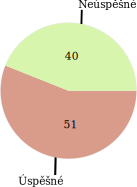
\includegraphics[width=0.28\textwidth]{../img/chart-succ.pdf}}
%     \hfill%
%     \subfloat[Graf zájmu o podobnou aplikaci.]%
%     {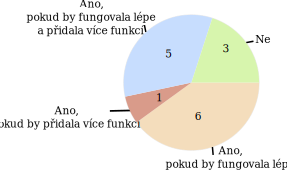
\includegraphics[width=0.6\textwidth]{../img/chart-interest.pdf}}
% \end{figure}

\newsavebox{\tempbox}
\begin{figure}[H]
    \sbox{\tempbox}{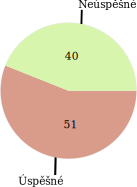
\includegraphics[width=0.28\textwidth]{../img/chart-succ.pdf}}
    \subfloat[Úspěšnost plnění.]{\usebox{\tempbox}\label{img-ratio-succ}}%
    \qquad
    \subfloat[Zájem o podobnou aplikaci.]{\vbox to \ht\tempbox{%
            \vfil
            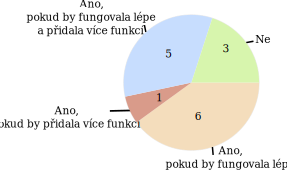
\includegraphics[width=0.6\textwidth]{../img/chart-interest.pdf}
            \vfil}\label{img-ratio-interest}}%
    \caption{Grafy výsledků.}
\end{figure}

Co se týká konkrétnějších důvodů nezdaru, největším problémem bylo nalezení více
kontaktů a nezdařený výběr z nich.